
%(BEGIN_QUESTION)
% Copyright 2006, Tony R. Kuphaldt, released under the Creative Commons Attribution License (v 1.0)
% This means you may do almost anything with this work of mine, so long as you give me proper credit

In your study of electronics, you probably learned that any amplifier can be turned into an {\it oscillator} by providing the right amount of phase-shifted feedback from output to input, with a minimum amount of total circuit gain.  This principle even had a name: the {\it Barkhausen criterion}.

$$\includegraphics[width=15.5cm]{i01459x01.eps}$$

So long as the product of the two gains is at least unity ($A_{amp} \cdot A_{feedback} \geq 1$), there will be sufficient amplification to sustain oscillation in the circuit.  One key to avoiding oscillation in such a circuit is to limit the total ``loop'' gain to less than unity.

\vskip 10pt

A process control system using feedback is not much different from this, and it too may oscillate if the total ``loop'' gain is excessive:

$$\includegraphics[width=15.5cm]{i01459x02.eps}$$

Describe what ``gain'' represents in each of the four components within the control system shown above ($A_C$, $A_{fce}$, $A_{process}$, and $A_T$), and identify which of these gains is easiest to alter.  Finally, explain how that one (easy-to-set) gain should be adjusted.  In other words, what criteria should determine its configured value?

\underbar{file i01459}
%(END_QUESTION)





%(BEGIN_ANSWER)

For each component in the control system, ``gain'' is defined in the same terms that gain is defined for any electronic component -- the ratio of output change to input change:

$$\hbox{Gain } = {\Delta \hbox{Out} \over \Delta \hbox{In}}$$

We may be more precise in our definition if we use calculus notation and express this ratio as a {\it derivative}:

$$\hbox{Gain } = {d \hbox{Out} \over d \hbox{In}}$$

As for how and why to set the controller gain at a particular value, I will let you discuss this with your classmates and arrive at your own answer!  I will say this, though: we do {\it not} want the system to break into oscillations!

\vskip 10pt

Challenge question: as you may (should!) recall, a necessary condition for oscillation in a feedback system is that the feedback be {\it positive}.  In other words, the phase shift from amplifier output to amplifier input needs to be 360$^{o}$, or else any oscillation will quickly die out due to interference, regardless of gain.  This being said, how can a control system ever oscillate, because we know the feedback is normally {\it negative} in nature, not positive?  Even if the controller gain were huge, shouldn't the inherently negative feedback of the system naturally prevent oscillation?

%(END_ANSWER)





%(BEGIN_NOTES)

Controller gain is obviously the easiest gain to set in a control system, and it should be set at a value great enough to provide quick, responsive control; but not so great that it causes the system to become unstable and oscillate.

\vskip 10pt

It is illustrative to have students generate the following gain equations for each of the four components shown in the process control loop (transmitter, controller, valve, and process):

$$\hbox{Transmitter Gain } = {\Delta \hbox{PV signal} \over \Delta \hbox{Measured variable}}$$

$$\hbox{Controller Gain } = {\Delta \hbox{MV signal} \over \Delta \hbox{PV signal}}$$

$$\hbox{Valve Gain } = {\Delta C_v \over \Delta \hbox{MV signal}}$$

$$\hbox{Process Gain } = {\hbox{Measured variable} \over \Delta C_v}$$

Note how the input of the next instrument in the loop comes from the output of the last!  This progression clearly shows the ``chain'' of information from one element to the other.

\vskip 10pt

In answer to the challenge question, negative feedback certainly would prohibit oscillation regardless of gain.  However, there will {\it always} be time lags in a feedback system, which mean that oscillation frequencies will be phase-shifted by those time lags.  At some frequency, every control system will develop an additional 180$^{o}$ of phase shift between controller output and controller input, thus turning what was originally negative feedback into positive feedback.  This, incidentally, is why feedback systems seek certain particular frequencies to oscillate at!  All other frequencies fail to generate the necessary phase shift for regenerative feedback, and thus die out.

%INDEX% Control, proportional: loop gain
%INDEX% Electronics review: Barkhausen criterion

%(END_NOTES)


